\documentclass{article} % For LaTeX2e
\usepackage{final_project,times}
\usepackage{amsmath, amssymb}
\usepackage{graphicx} % To include figures
\usepackage{caption}
\usepackage{subcaption}
\usepackage{epstopdf}
\usepackage{hyperref}
%\documentstyle[nips12submit_09,times,art10]{article} % For LaTeX 2.09






\title{COMPSCI 571 Final Project Report}


\author{
Hangjie Ji$^1$, Yuhao Hu$^1$, Guoshan Liu$^2$, Ma Luo$^1$\\
$^1$Department of Mathematics, $^2$Department of Electrical and Computer Engineering\\
Duke University\\
Durham, NC 27708 \\
\texttt{yh89@duke.edu} \\
}

\newcommand{\fix}{\marginpar{FIX}}
\newcommand{\new}{\marginpar{NEW}}

\nipsfinalcopy

\def\R{\mathbb{R}}


\begin{document}



\maketitle

\begin{abstract}
      With an available piece of dataset concerning online news (see \cite{FVC14}), 
      the methods of random forest with bagging and Principal Component Analysis (PCA) are used to 
      investigate the relation among the news-features . In particular, while \cite{FVC14} gave predictions for the popularity of online news in general, we
      obtain predicators for online news from various channels (e.g., lifestyle, world, etc.) with comparable accuracy. On the other hand, we use the features 
      other than those relevant to the channel information to classify which channel a particular piece of online news is most likely to be from. This workes well for
      four of the six available channels, noting that all the features are numerical and contain no information about, say, explicit keywords of the news.
\end{abstract}

\section{Introduction}
Given a piece of online news, is it possible to predict its popularity by knowing its channel, publishing time, its title length and the number of images or videos in it, etc?
In aswering to this, K. Fernandes, P. Vinagre and P. Cortez \cite{FVC14} designed a decision support system using the random forest model applied to a dataset of 39797 news websites and their corresponding 61 features, which includes all the features which we mentioned above. 

In the current work, we further the investigation, using the same dataset, based on the following two questions: 

\begin{itemize}
\item{How does channel affect popularity? How to compare a predictor trained restricting to a specific channel to one trained with the entire dataset? }
\item{Do channels have ``styles"? In other words, is it possible to learn the channel (``Lifestyle",``Entertainment",``Business",``Social Media",``Tech",``World") using all  the other features?}
\end{itemize}

To answer the first question, we apply a version of random forest algorithm to each subset of the data that belong to a specific channel. In each channel category, popularity is defined as a binary function so
that the distinction between popular/unpopular is balanced.
In question two, a possible restriction from the dataset is that all values in the data are numerical, thus one cannot make use of the explicit keywords of the news, which may be of valuable information to help
classify which channel a piece of news belong. In both tasks, we experiment with the method of Principal Component Analysis(PCA) to reduce the dimension of the data.

\section{Methods}
In this section, we introduce the two main methods used in the current project: {\it Principal Component Analysis}, and {\it Random Forest with Bagging}.
\subsection{PCA}

The method of Principal Component Analysis (PCA), an effective tool in reducing the dimensions of data, is based on the following well-known singular-value
decomposition theorem:
\\

\textbf{Theorem.} For any $m\times n$ matrix $A$, there exist orthogonal matrices $U,V$ and a 
diagonal $m\times n$ matrix $\Sigma$, such that
			\[
				A = U\Sigma V^T,
			\]
where the diagonal entries of $\Sigma$ are non-negative arranged decreasingly.	
\\

The following theorem tells one how to use the Singular-Value Decomposition Theorem:
\\

\textbf{Theorem.} Let $A$ be an $m\times n$ matrix of $n$ data points in $\R^m$, centered (i.e., $\mu(A)\textbf{1}_n^T = 0$). Assuming $n>m$. Let $\sigma_1,...,\sigma_m$ be the $m$ singular
values of $A$, coming from its SVD, namely $U\Sigma V^T$. Let $k<m$ be any integer. Then the columns of the matrix $U_kA$, where $U_k = U(:, 1:k)$ satisfies the following:
\begin{itemize}
	\item{They are vectors in $\R^k$, where $k<m$;}
	\item{They are uncorrelated;}
	\item{They obtain the dimensions of greatest variance in $A$.}
\end{itemize}
\
In practice, say, the prediction of popularity, we exclude the ``time/date" and ``share number" features, and carry out the PCA on the remaining 59 features. Empirically, choosing $k$ between 15-35 gave
better prediction results.

				

\subsection{Random Forest with Bagging}
Consider a dataset $\{(X_i, y_i)\}$ in which the $X_i$ and $y_i$ stand for the features and labels, respectively. A {\it classification tree} $T$ is a procedure that
 takes a feature $X$ as input and outputs the posterior probability distribution $p(y|X)$ of the labels given $X$. In particular, a classification tree can have the
 following construction:  The tree $T$ is binary, where each non-leaf node has two children $T_L, T_R$. At each tree node, one restores a positive integer $d$, and a real 
 number $t$. All the features starts from the root of the tree and start splitting according to the rule:
 			\[
				L = \{(X,y)|x_d\le t\}, \qquad R = \{(X,y)|x_d>t\}.
			\]
That is, passing through each node, we look at the $d$-th dimension of a feature $X$ and decide to descend to the right or left child of the tree according to whether
this value is greater or less than $t$.
\\

Of course, the performance of a classification tree is affected by the parameters that one choose for the construction of the tree, including its maximum depth. (Note: If
the depth of the tree is too large, one would more likely to end up overfitting the data.) One way of choosing the parameters is called ``optimal splitting". The idea is 
to maximize the reduction of training error in each splitting of the features. First note that each tree node $\tau$ maintains the probability distribution $p(y|S_\tau)$,
where $S_\tau$ are the training data which classified to $\tau$. One 
could thus define the {\it impurity}:
			\[
				i(S_\tau) = 1-\max_y p(y|S_\tau). 
			\]
The decrease in training error is simply measured by
			\[
				\Delta i(S_\tau,S_{\tau.L}, S_{\tau.R}) = i(S_\tau) - \frac{|S_{\tau.L}|}{|S_\tau|}i(S_{\tau.L})-\frac{|S_{\tau.R}|}{|S_\tau|}i(S_{\tau.R}).
			\]			
For each note, we iterate through all $d$ and $t$ so that $\Delta i(S_\tau,S_{\tau.L}, S_{\tau.R}) $ is maximized.
\\

Another way of choosing the classification tree parameters is to randomize them. To make this effective, it is advisable to consider a number of such trees
and let them vote. This algorithm is what's named {\it random forest}. In practice, the result can be improved by considering in addition training each tree with
randomly selected (with replacement) training samples in $\{(X_i,y_i)\}$.  This is what we use in the current work. 
\\

For more discussion on random forest with bagging, see \cite{breiman2001random, breiman1996bagging}.
\subsection{Error Measurement}
For the two tasks we mentioned above, we adapt similar error measurements for either the popularity (binary) of the news.

Popularity Prediction:
\begin{itemize}
\item {Recall}:$\displaystyle{\frac{TP}{R}} = \displaystyle\frac{TP}{TP+FN}$
\item {Specificity/Sensitivity}:$\dfrac{TN}{I} = \displaystyle\frac{TN}{FP+TN}$
\item {Precision}:$\dfrac{TP}{P} = \displaystyle\frac{TP}{TP+FP}$
\\
\end{itemize}

Channel Classification:
\begin{itemize}
\item $C_i = \text{ data classified on channel } i$
\item $T_i = \text{ data whose true channel is } i$
\item $\text{score }(i) = \displaystyle\frac{\#(C_i \cap T_i)}{\# T_i},$ $\qquad \text{precision }(i) = \displaystyle\frac{\#(C_i \cap T_i)}{\# C_i}$
\\
\end{itemize}




\section{Results}
\subsection{Popularity Prediction by Channels}

Applying the methods above to the 59 features (excluding ``date/time" and ``sharing rate"), we obtain a trained forest for each of the six categories of data. For each category (``channel"), the training is
done on half of the data, randomly selected, then tested on the remaining half. The training accuracy is shown in Figure \ref{pop} in the Appendix, plotted against the number of trees used in a random forest. 

\subsection{Inference of the ``Channel" feature}

For the entire data, we consider maintaining only the features irrelevant to ``date/time" and the channel information, counting 52. PCA with $k = 25$ is applied. Training is done on half of the dataset, randomly
chosen. Random forest with 80 trees is applied for optimal results. Testing is carried out on the remaining half of the data, yielding accuracy results plotted in Figure \ref{channelBar}. For an intuitive representation of the result, see
Figures \ref{channelScore} and  \ref{channelPres} in the Appendix.
\\

As a conclusion, after applying the PCA for dimension reduction and Random Forest with bagging for training, we could, quite surprisingly classify the channels of four categories of the news (Business, Social Media,
Technology and World) with both measurements of error (score and precision) to be above $70\%$. Measurement with either score or precision (only one) could have even more optimal outcomes. 
\\

Finally, it is worth
noting that the classification is done without knowing explicitly any of the key words that may appear frequently in news belonging to a specific channel. Thus, we would expect better results of training with this 
information. On the other hand, one might also ask why certain channels are harder to classify. Is it because they share some similarity, in terms of the available features, with some other channels? We will leave 
answers to these questions to future investigations. See the Discussion section for more questions like this.

\begin{figure}[h!]
	\centering
	\includegraphics[scale = 0.5]{precision.pdf}
	\caption{Accuracy of Inference of Channel}
	\label{channelBar}
\end{figure}



\section{Discussion}

For further investigation, the following questions may be worth considering:
\begin{itemize}
	\item For channel classification, improve the accuracy with keywords (or other relevant) information.
	\item Find out why our current channel classification works not as well for two of the six channels, namely, ``lifestyle" and ``social media". 
	\item For different random forest sizes, the prediction rates display certain patterns. Find an explanation for these patterns.
	\item Improve the prediction accuracy for news popularity, for a specific channel or in general.
\end{itemize}




\section{Acknowledgement}

We thank the authors of \cite{FVC14} for making  their data available through the link: 

\url{https://archive.ics.uci.edu/ml/datasets/Online+News+Popularity}

\bibliographystyle{amsalpha}
\bibliography{MLProj}





\newpage

\section{Appendix}
\vskip 1.5cm
\begin{figure}[h!]
\centering
 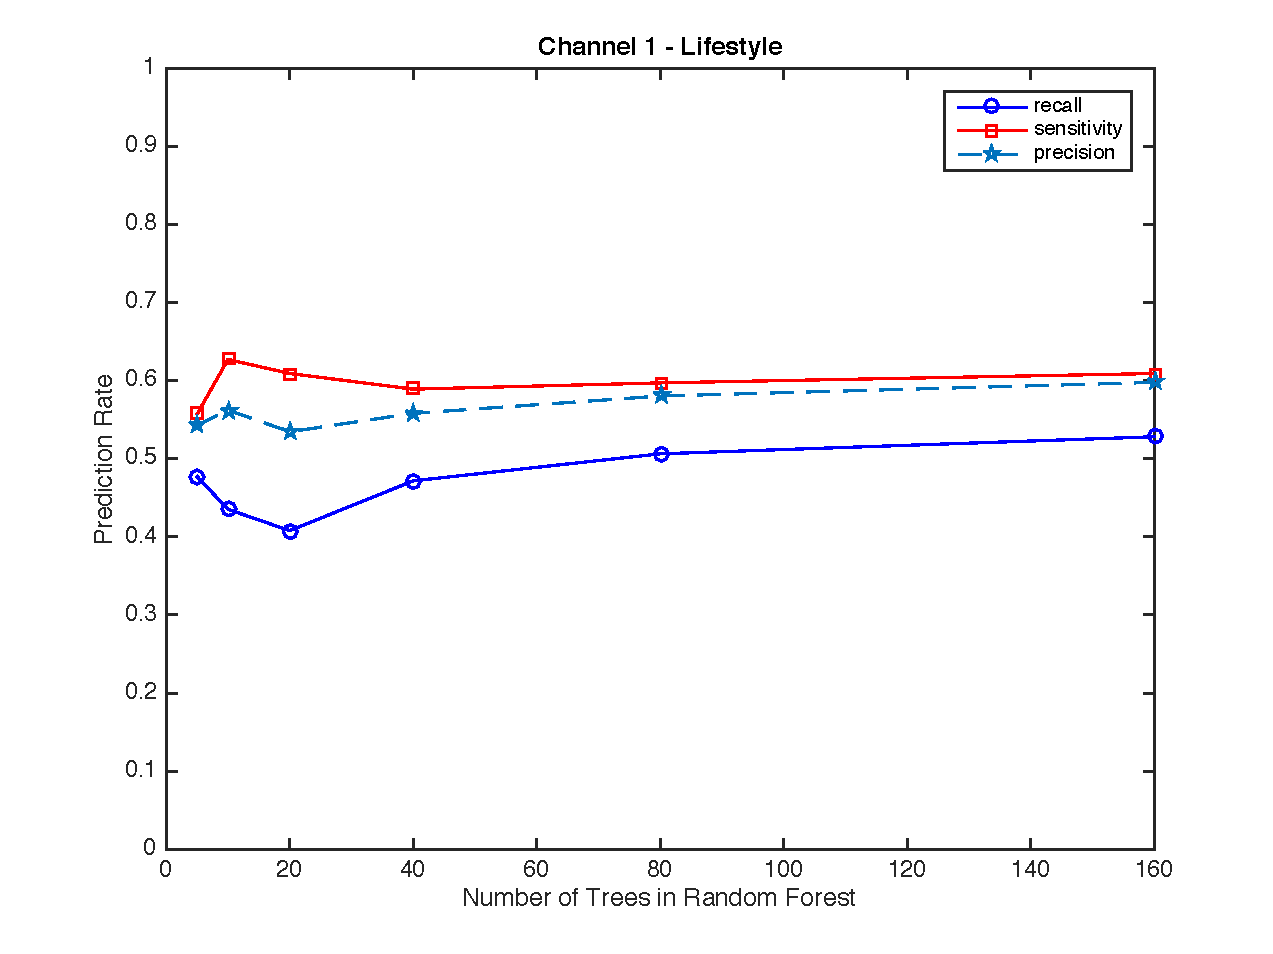
\includegraphics[scale = 0.32]{channel_1.pdf}
 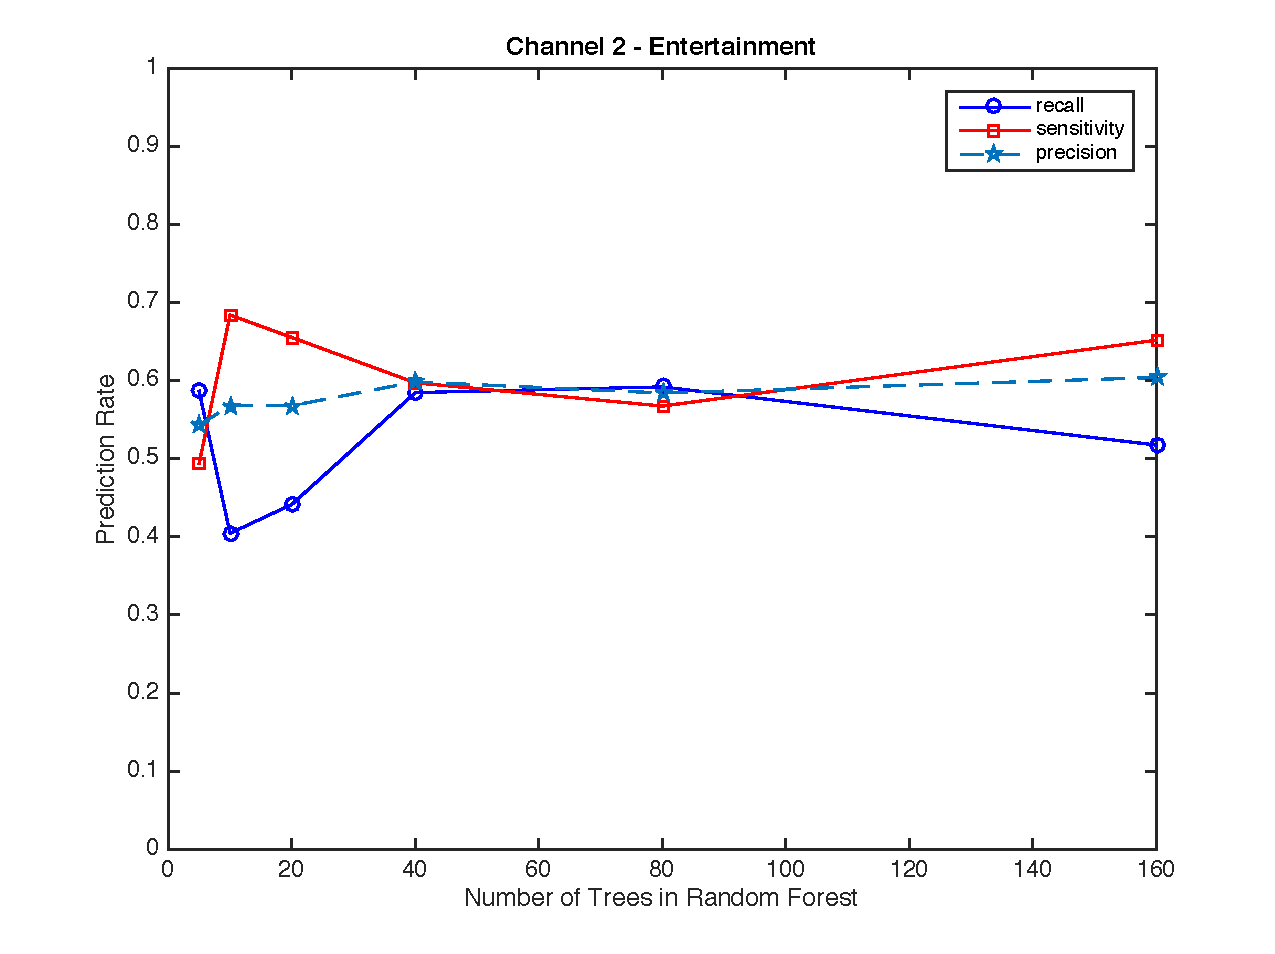
\includegraphics[scale = 0.32]{channel_2.pdf}
 \includegraphics[scale = 0.35]{channel_3.pdf}
 \includegraphics[scale = 0.35]{channel_4.pdf}
 \includegraphics[scale = 0.35]{channel_5.pdf}
 \includegraphics[scale = 0.35]{channel_6.pdf}
 \caption{Popularity Prediction for Each Channel Category}
 \label{pop}
\end{figure}

\begin{figure}[h!]
\centering
 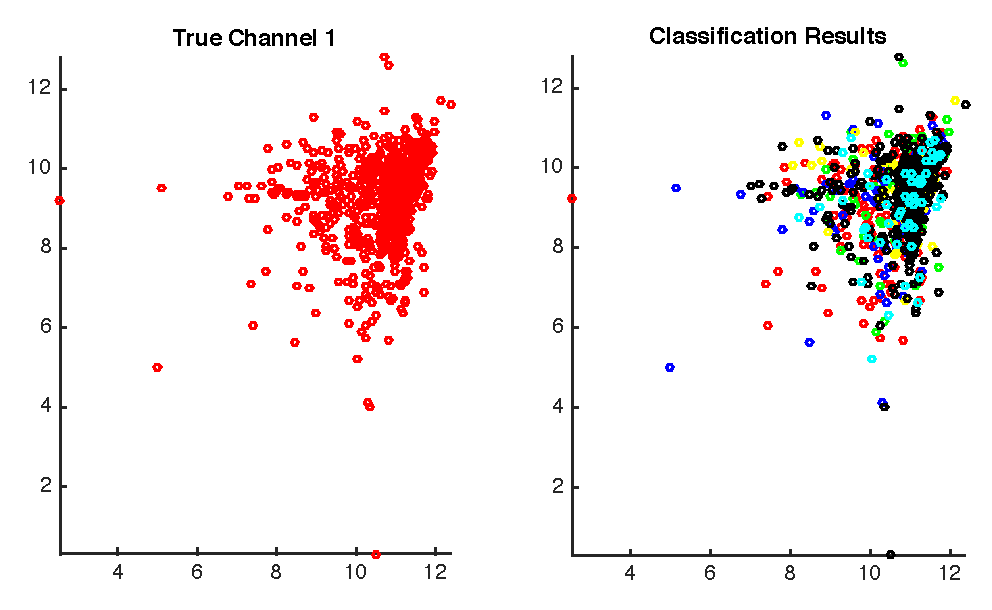
\includegraphics[scale = 0.4]{scoreFig1.pdf}\hspace{0.5cm}
 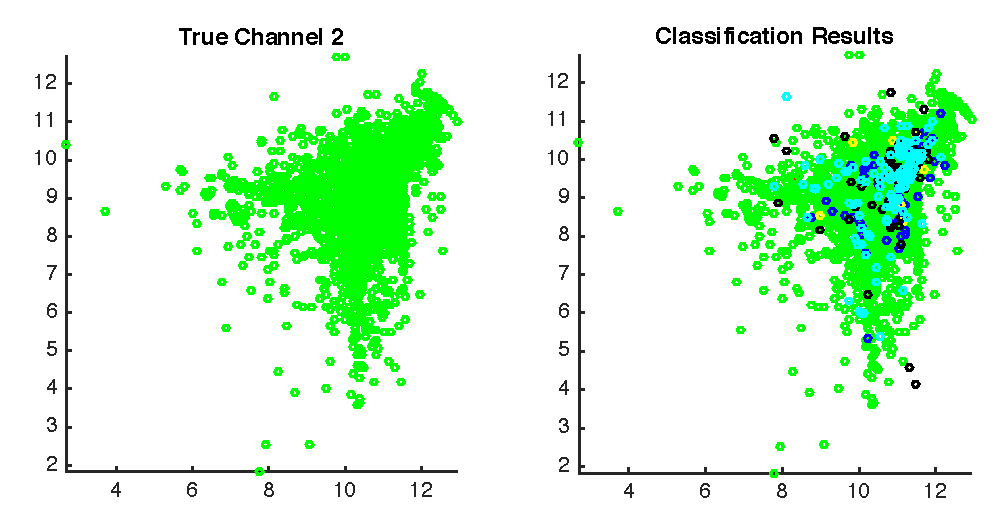
\includegraphics[scale = 0.4]{scoreFig2.pdf}
 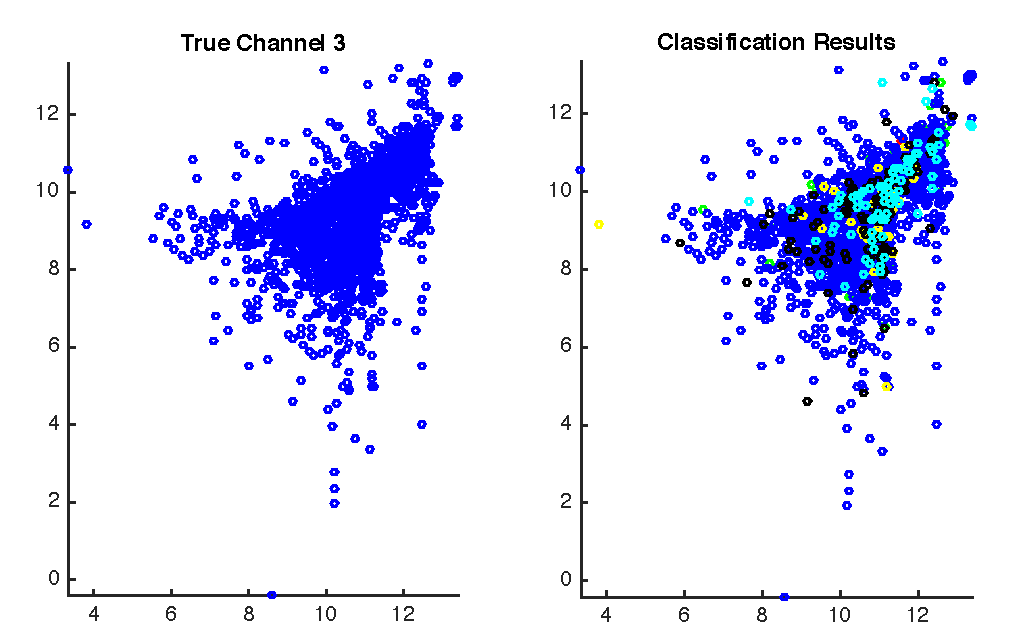
\includegraphics[scale = 0.4]{scoreFig3.pdf}\hspace{0.5cm}
 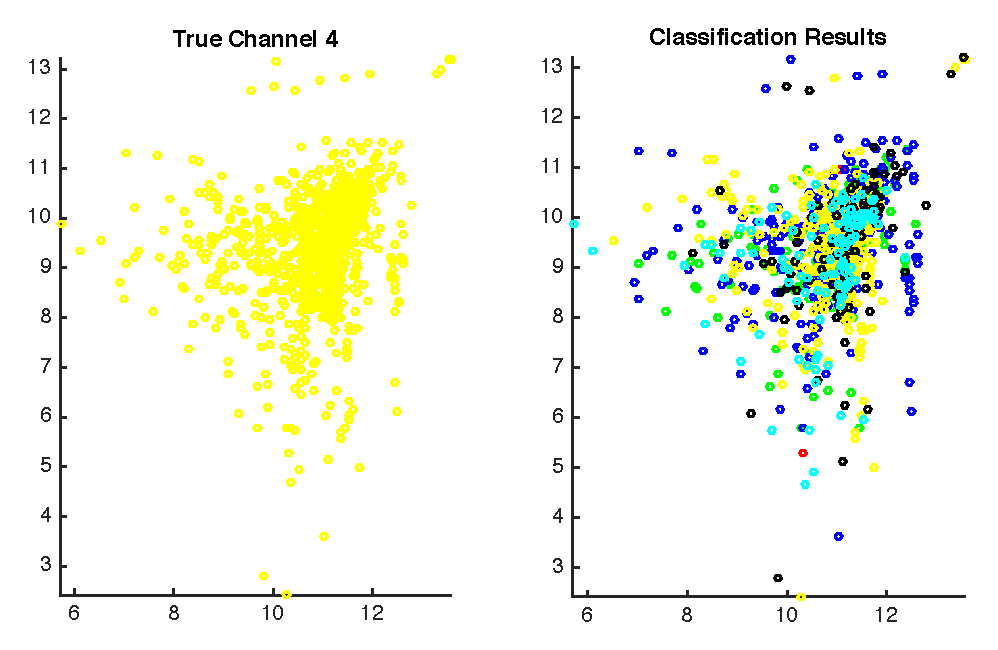
\includegraphics[scale = 0.4]{scoreFig4.pdf}
 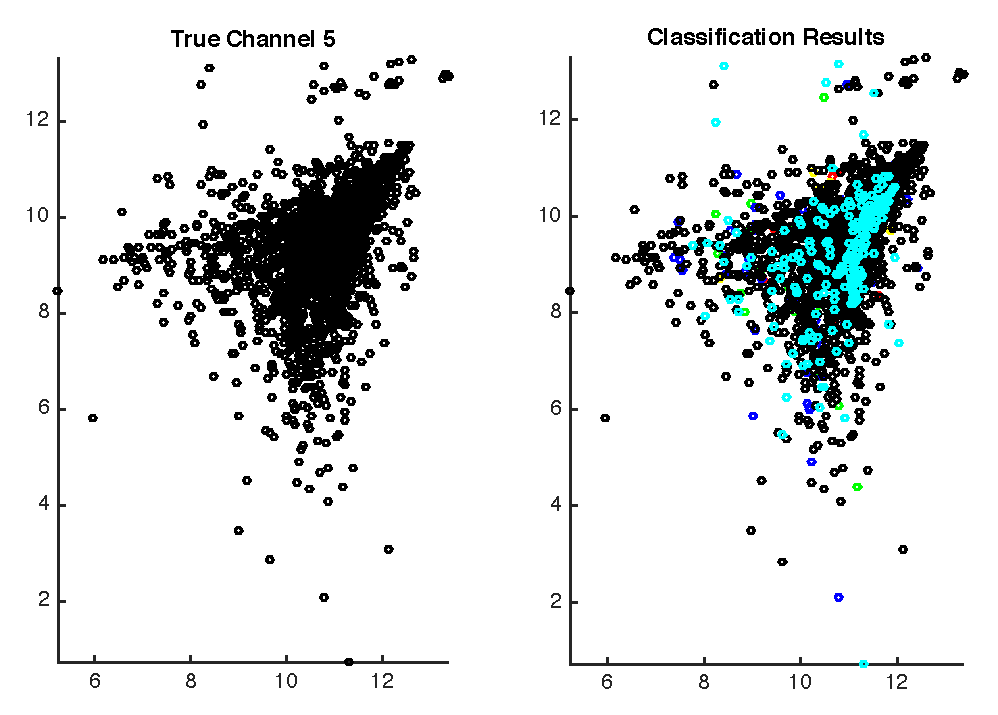
\includegraphics[scale = 0.4]{scoreFig5.pdf}\hspace{0.5cm}
 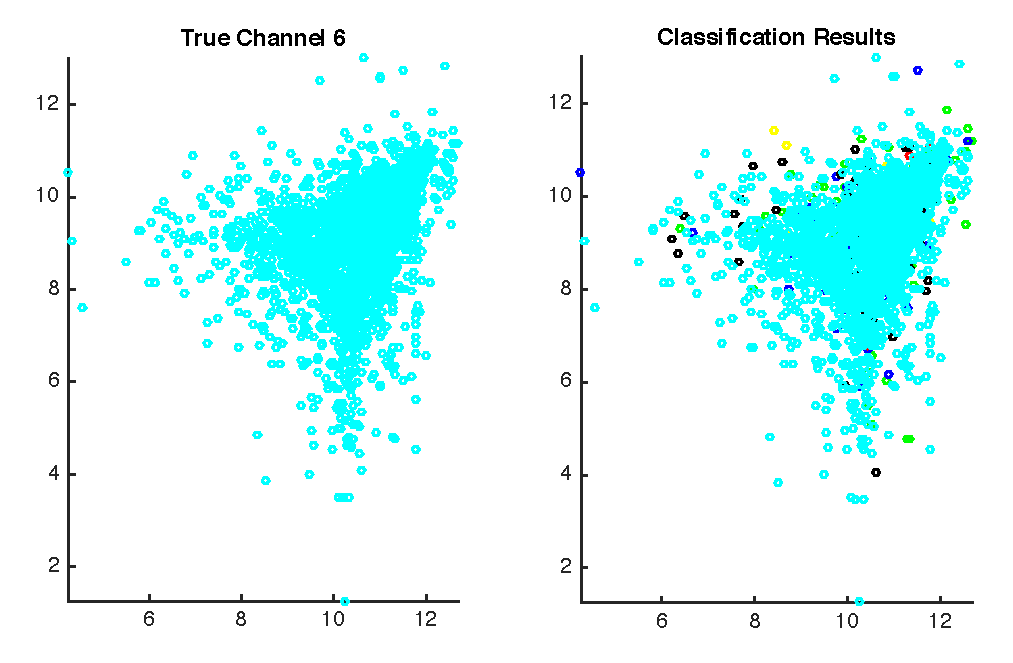
\includegraphics[scale = 0.4]{scoreFig6.pdf} 
 \caption{Inference of Channel, Score}
 \label{channelScore}
\end{figure}



\begin{figure}[h!]
\centering
 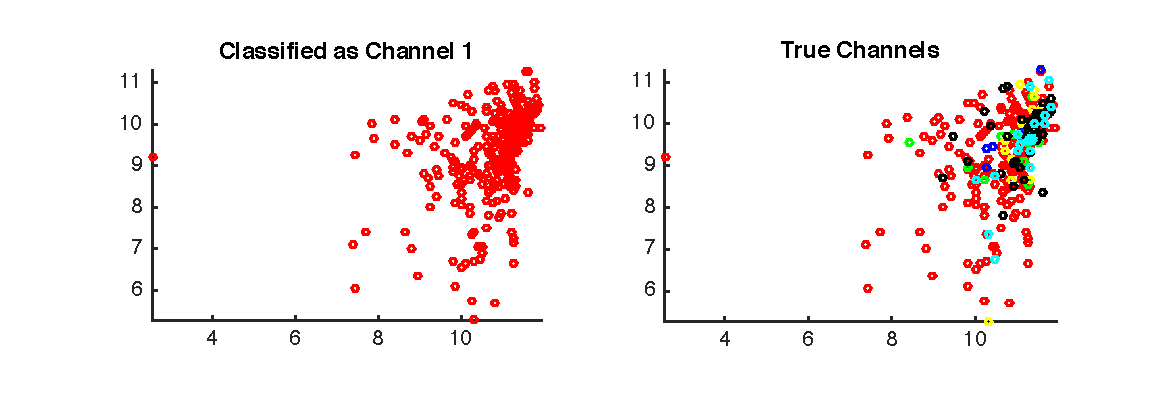
\includegraphics[scale = 0.4]{precisionFig1.pdf}\hspace{0.5cm}
 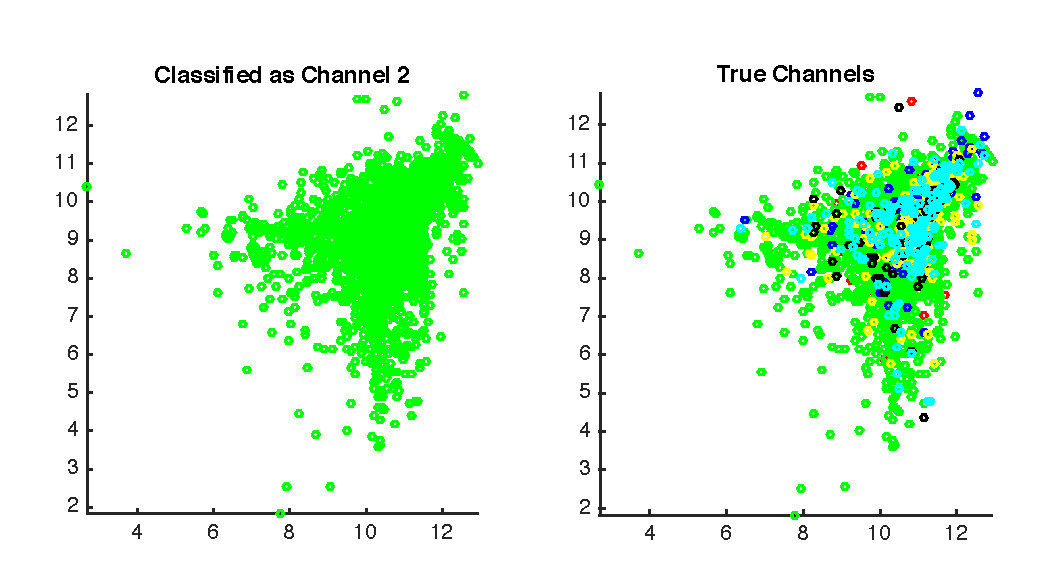
\includegraphics[scale = 0.4]{precisionFig2.pdf}
 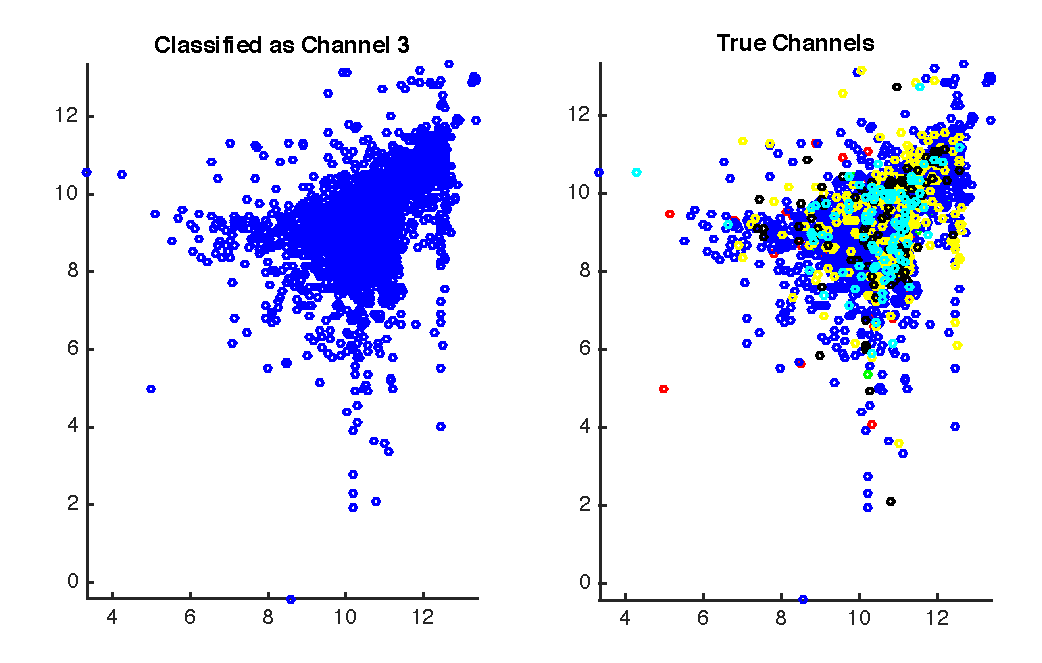
\includegraphics[scale = 0.38]{precisionFig3.pdf}\hspace{0.5cm}
 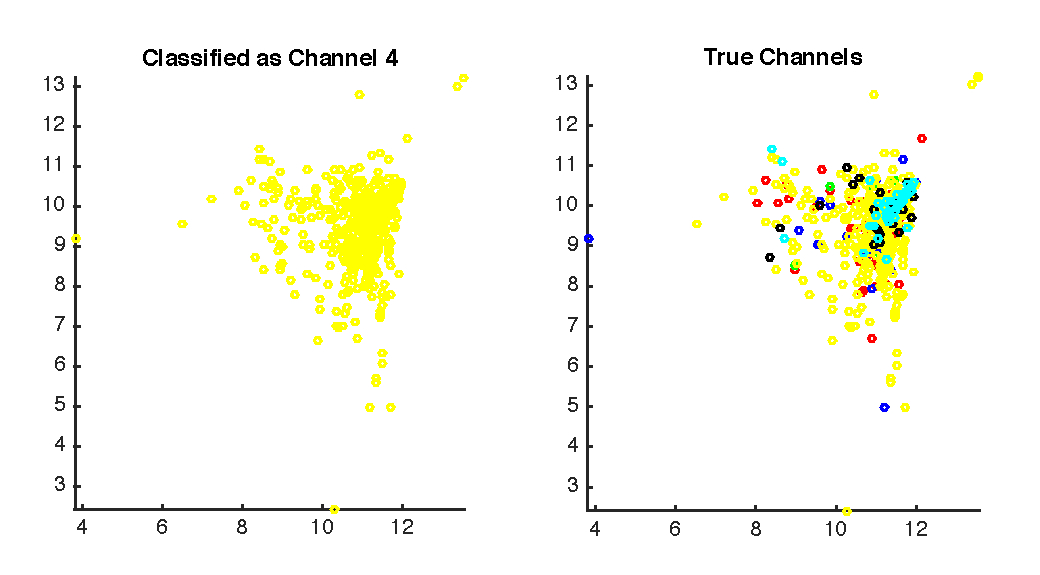
\includegraphics[scale = 0.4]{precisionFig4.pdf}
 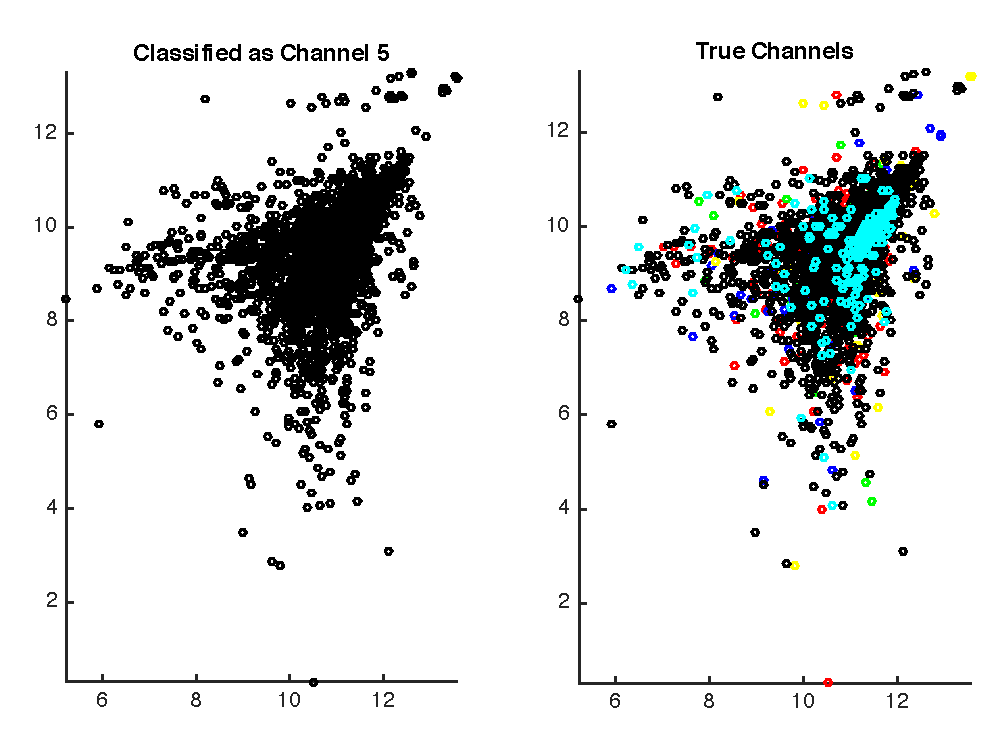
\includegraphics[scale = 0.38]{precisionFig5.pdf}\hspace{0.5cm}
 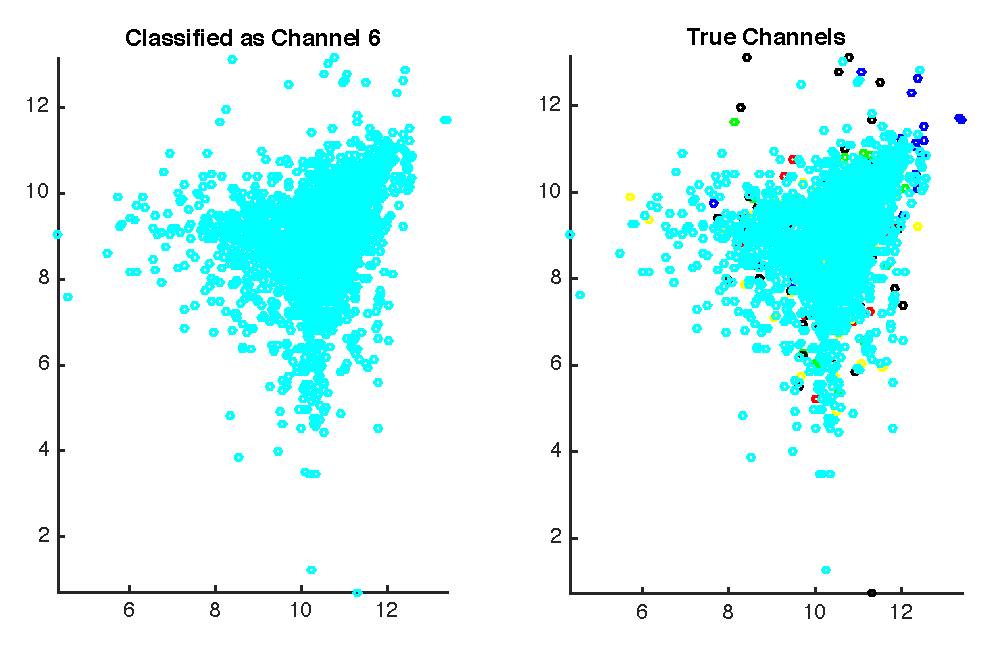
\includegraphics[scale = 0.4]{precisionFig6.pdf} 
 \caption{Inference of Channel, Precision}
 \label{channelPres}
\end{figure}





\end{document}
